\documentclass[sigconf]{acmart}

\usepackage{graphicx}
\usepackage{caption}
\usepackage{subcaption}
\usepackage{mathtools}
\usepackage{algpseudocode}
\usepackage{algorithm}
\usepackage{algorithmicx}
\usepackage{graphicx}
\usepackage{hyperref}
\usepackage{textcomp}



%\usepackage{booktabs} % For formal tables


\copyrightyear{2017} 
\acmYear{2017} 
\setcopyright{acmlicensed}
\acmConference[CEE-SECR '17]{Central and Eastern European Software Engineering Conference Russia}{October 20--21, 2017}{Saint-Petersburg, Russian Federation}
%\acmBooktitle{CEE-SECR '17: Central and Eastern European Software Engineering Conference Russia, October 20--21, 2017, Saint-Petersburg, Russian Federation}
\acmPrice{15.00}
\acmDOI{10.1145/3166094.3166104}
\acmISBN{978-1-4503-6396-9/17/10}

%Conference
%%\acmConference[SECR'17]{Software Engineering Conference Russia}{October 2017}{St. Petersburg, Russia} 
%%\acmYear{2017}
%%\copyrightyear{2017}

%\acmPrice{15.00}


\begin{document}

\newtheorem{mytheorem}{Theorem}

\algrenewcommand\algorithmicindent{0.5em}
\algnewcommand\algorithmicswitch{\textbf{switch}}
\algnewcommand\algorithmiccase{\textbf{case}}
\algnewcommand\algorithmicassert{\texttt{assert}}
\algnewcommand\Assert[1]{\State \algorithmicassert(#1)}
% New "environments"
\algdef{SE}[SWITCH]{Switch}{EndSwitch}[1]{\algorithmicswitch\ #1\ \algorithmicdo}{\algorithmicend\ \algorithmicswitch}
\algdef{SE}[CASE]{Case}{EndCase}[1]{\algorithmiccase\ #1}{\algorithmicend\ \algorithmiccase}

\algtext*{EndSwitch}
\algtext*{EndCase}
\algtext*{EndWhile}% Remove "end while" text
\algtext*{EndIf}% Remove "end if" text
\algtext*{EndFor}% Remove "end for" text
\algtext*{EndFunction}% Remove "end function" text

\newif\ifboldnumber
\newcommand{\boldnext}{\global\boldnumbertrue}

% Default definition is \footnotesize#1:
\algrenewcommand\alglinenumber[1]{%
  \footnotesize\ifboldnumber\bfseries\fi\global\boldnumberfalse#1:}


\title[CFPQ with Structural Representation of Result]{Context-Free Path Querying with Structural Representation of Result}
%\titlenote{Produces the permission block, and
%  copyright information}
%\subtitle{Extended Abstract}
%\subtitlenote{The full version of the author's guide is available as
%  \texttt{acmart.pdf} document}


\author{Semyon Grigorev}
\affiliation{%
  \institution{Saint Petersburg State University}
  \streetaddress{7/9 Universitetskaya nab.}
  \city{St. Petersburg} 
  \state{Russia} 
  \postcode{199034}
}
\email{semen.grigorev@jetbrains.com}

\author{Anastasiya Ragozina}
\affiliation{%
  \institution{Saint Petersburg State University}
  \streetaddress{7/9 Universitetskaya nab.}
  \city{St. Petersburg} 
  \state{Russia} 
  \postcode{199034}
}
\email{ragozina.anastasiya@gmail.com}


% The default list of authors is too long for headers}
%\renewcommand{\shortauthors}{B. Trovato et al.}


\begin{abstract}
Graph data model and graph databases are popular in such areas as bioinformatics, semantic web, and social networks.
One specific problem in the area is a path querying with constraints formulated in terms of formal grammars.
The query in this approach is written as a grammar and paths querying is graph parsing with respect to the grammar.
There are several solutions to it, but they are based mostly on CYK or Earley algorithms which impose some restrictions in comparison with other parsing techniques, and employing of advanced parsing techniques for graph parsing is still an open problem.
In this paper we propose a graph parsing technique which is based on generalized top-down parsing algorithm (GLL) and allows one to build finite structural query result representation with respect to the given grammar in polynomial time and space for arbitrary context-free grammar and graph.
\end{abstract}

%
% The code below should be generated by the tool at
% http://dl.acm.org/ccs.cfm
% Please copy and paste the code instead of the example below. 
%
\begin{CCSXML}
<ccs2012>
<concept>
<concept_id>10002951.10002952.10002953.10010146</concept_id>
<concept_desc>Information systems~Graph-based database models</concept_desc>
<concept_significance>500</concept_significance>
</concept>
<concept>
<concept_id>10002951.10002952.10003197.10010825</concept_id>
<concept_desc>Information systems~Query languages for non-relational engines</concept_desc>
<concept_significance>500</concept_significance>
</concept>
<concept>
<concept_id>10003752.10003766.10003771</concept_id>
<concept_desc>Theory of computation~Grammars and context-free languages</concept_desc>
<concept_significance>300</concept_significance>
</concept>
<concept>
<concept_id>10011007.10011006.10011041.10011688</concept_id>
<concept_desc>Software and its engineering~Parsers</concept_desc>
<concept_significance>300</concept_significance>
</concept>
</ccs2012>
\end{CCSXML}

\ccsdesc[500]{Information systems~Graph-based database models}
\ccsdesc[500]{Information systems~Query languages for non-relational engines}
\ccsdesc[300]{Theory of computation~Grammars and context-free languages}
\ccsdesc[300]{Software and its engineering~Parsers}

\keywords{Graph database, path query, graph parsing, CFPQ, context-free grammar, top-down parsing, GLL, LL}

%\acmBadgeR{artifacts_available}

\maketitle

\section{Introduction}
Graph data model and graph data bases are very popular in such areas as bioinformatics, semantic web, and social networks.
Hence, different graph structured data analysis problems are stated and appropriate solutions for these problems are required.
%Extraction of paths which satisfy specific constraints may be useful for investigation of graph structured data and for detection of relations between data items.
One specific problem---path querying with constraints---is usually formulated in terms of formal grammars and is called formal language constrained path problem~\cite{FLCpathProblem}.

Classical parsing techniques can be used to solve formal language constrained path problem and thus the more common problem---graph parsing. 
Graph parsing may be required in graph data base querying, formal verification, string-embedded language processing, and any other areas where graph structured data is used. 

%Though constrains formulated in terms of regular languages is widely used, using of more powerful context-free grammars for graph querying is in active research: recent results is context-free extension for SPARQL~\cite{CFGonRDF} and research of Jelle Hellings~(\cite{Hellings16,ConjCFPathQuery}).

Existing solutions in context-free graph querying field usually employ such parsing algorithms as CYK or Earley~(for example~\cite{ConjCFPathQuery,CFGonRDF,GraphQueryWithEarley}). 
These algorithms are simple, but impose restrictions.
For example, CYK algorithm demands the input grammar to be transformed into Chomsky normal form causing performance issues, since parsing time depends on grammar size which significantly increases during the transformation.
Such algorithms as GLR and GLL process arbitrary context-free grammars, thus performance may be improved by employing them for graph parsing problem.
%Moreover, Earley-based graph parsing algorithm, which proposed in~\cite{GraphQueryWithEarley}, has restrictions on processing graphs with cycles: it is required to specify maximal length of path for parsing termination.
Other properties of parsing algorithms also affect performance: for example, in~\cite{Hellings16} author expects that it is possible to improve evaluation of queries for a given pair of nodes by using top-down directed parsing algorithm.
Both CYK and Earley parsing algorithms are bottom-up, CYK is undirected, and Earley-based implementation~\cite{GraphQueryWithEarley} is known to have issues with cycles processing. 
In this paper we show this assumption is true.
We also provide a positive answer to the question of applicability of advanced parsing techniques stated in~\cite{Hellings16}.
%The applicability of advanced parsing techniques~\cite{Grune} for path querying is stated as an open question in~\cite{Hellings16} and we provide positive answer to it.

Even though a set of path querying solutions has been developed~\cite{GraphQueryWithEarley,ConjCFPathQuery,QueryGraphWithData,RegularDBQuery}, query result exploration is still a challenge~\cite{hofman2015separabilityForRegQueryDebugging}, as also there is a need for simplification of complex query debugging, especially for context-free queries.
In~\cite{Hellings16}, annotated grammars are proposed as a possible solution: this representation is finite for any input data and contains information necessary for detailed result exploration.
In the paper we propose the representation more native for grammar based analysis, provided by classical parsing techniques---derivation tree---which contains exhaustive information about parsed sentence structure in terms of specified grammar.

We make the following contributions in this paper.
\begin{enumerate}
\item We propose the graph parsing algorithm based on the generalized top-down parsing algorithm---GLL~\cite{scott2010gll}---and provide its time and space complexity estimations. 
For graph $M=(V,E,L)$, space complexity is $O(|V|^3 + |E|)$ and time complexity is $O\left(|V|^3*\max\limits_{v \in V}\left(deg^+\left(v\right)\right)\right)$.
\item We answer some questions on advanced parsing techniques applicability for graph processing stated in~\cite{Hellings16}.
%Questions on possibility of advanced parsing techniques application for graph processing, and on possibility of top-down algorithms utilization for  answering queries for a given pair of nodes are stated in~\cite{Hellings16}.
%We show that all of these are possible.
%Thus we answer on first and second questions which are stated in~\cite{Hellings16}: yes, we can use advanced parsing techniques for graph parsing, and we can use top-down parsing algorithm for goal-oriented queries evaluation.
\item Proposed graph parsing algorithm constructs finite representation of parse forest containing derivation trees for all matched paths in graph. We show how this representation can be used for realistic problems solving.
\item We have implemented the proposed algorithm and our evaluation shows that advanced parsing techniques increase performance (up to 1000 times in some cases) as compared to CYK-based implementation, proposed in~\cite{CFGonRDF}.
\end{enumerate}

\section{Preliminaries}

In this work we are focused on the parsing algorithm, and not on the data representation, and we assume that whole input graph can be optimally located in RAM memory.

We start by introduction of necessary definitions.
\begin{itemize}
  \item Context-free grammar is a quadruple $G=(N, \Sigma, P, S)$, where $N$ is a set of nonterminal symbols, $\Sigma$ is a set of terminal symbols, $S \in N$ is a start nonterminal, and $P$ is a set of productions. 
  \item $\mathcal{L}(G)$ denotes a language specified by grammar $G$, and is a set of terminal strings derived from start nonterminal of $G$: $L(G) = \{\omega | S \Rightarrow_{G}^{*} \omega\}$.
  \item Directed graph is a triple $M = (V,E,L)$, where $V$ is a set of vertices, $L \subseteq \Sigma$ is a set of labels, and a set of edges $E\subseteq V\times L\times V$. 
  We assume that there are no parallel edges with equal labels: for every $e_1=(v_1,l_1,v_2) \in E, e_2=(u_1,l_2,u_2) \in E$ if $v_1 = u_1$ and $v_2 = u_2$ then $l_1 \neq l_2$.
  \item $tag: E \rightarrow L$ is a helper function which returns a tag of a given edge. $$tag(e = (v_1,l,v_2), e \in E) = l$$
  \item $\oplus: L^+ \times L^+ \rightarrow L^+$ denotes tag concatenation operation.
%  \item Path $p$ in graph $M$ is a list of incident edges: 
%  \begin{align*}
%   p &= e_0,e_1,\dots,e_{n-1} \\
%     &= (v_0,l_0,v_1),(v_1,l_1,v_2),\dots,(v_{n-1},l_{n-1},v_n)
%  \end{align*}
%  where $v_i \in V$, $e_i \in E$, $e_i=(v_i,l_i,v_{i+1})$, $l_i \in L$, $|p| = n, n \geq 1$. 
%  \item $P$  is a set of paths $\{p: p \text{ path in } M\}$, where $M$ is a directed graph.
%  \item $\Omega: P \rightarrow L^+$ is a helper function which constructs a string produced by the given path. For every $p \in P$
  \item $\Omega$ is a helper function which constructs a string produced by the given path. For every $p \text{ path in } M$
  $$ \Omega(p = e_{0},e_{1},\dots,e_{n-1}) = tag (e_{0}) \oplus \dots \oplus tag (e_{n-1}).$$
\end{itemize}

Using these definitions, we define context-free language constrained path querying as, given a query in form of grammar $G$, to construct the set of paths $$Q(M,G)=\{p|p \text{ is path in } M, \Omega(p) \in \mathcal{L}(G)\}.$$

Note that $Q(M, G)$ can be an infinite set, hence it cannot be represented explicitly. 
In order to solve this problem, we construct compact data structure representation which stores all elements of $Q(M,G)$ in finite space and from which one can extract any of them.

\subsection{Generalized LL Parsing Algorithm}\label{BasicGLL}

One of widely used classes of parsing algorithms is LL(k)~\cite{Grune}---top-down algorithms which read input from left to right, build leftmost derivation, and use $k$ symbols for lookahead.
LL(k) parser may be implemented as deterministic pushdown automaton (DPDA).
On the other hand, LL(k) parser may be implemented in recursive-descent manner: each rule transforms to function which can call functions for other rules in order specified by right hand side of corresponded rule.
In this case, stack of DPDA is replaced with functions call stack.

Classical LL algorithm operates with a pointer to the input (position $i$) and a grammar slot---pointer to the grammar of form $N \rightarrow \alpha \cdot x \beta $.
Parsing may be described as a transition system from the initial state ($i = 0$, $S \rightarrow \cdot \beta $, where $S$ is start nonterminal) to the final ($i = input.Length$, $s \rightarrow \beta \cdot$).
At each step, there are four possible cases. 

\begin{enumerate}
\item $N \rightarrow \alpha \cdot x \beta $, when $x$ is a terminal and $x = input[i]$. In this case both pointers should be moved to the right ($i \leftarrow i + 1$, $N \rightarrow \alpha  x \cdot \beta $).
\item $N \rightarrow \alpha \cdot X \beta $, when $X$ is nonterminal. In this case we push return address $N \rightarrow \alpha X \cdot \beta $ to the stack and move pointer in the grammar to position $X \rightarrow \cdot \gamma$.\label{itm:2}
\item $N \rightarrow \alpha \cdot $. This case means that processing of nonterminal $N$ is finished. We should pop return address from stack and use it as a new slot.\label{itm:3}
\item $S \rightarrow \alpha \cdot $, where $S$ is a start nonterminal of grammar. In this case we should report success if $i = input.Length - 1$ or failure otherwise. 
\end{enumerate}

There can be several slots $X \rightarrow \cdot \gamma$ in the second case since the algorithm is nondeterministic, so some strategy to choose one of them for further parsing is needed.
Lookahead is used to avoid nondeterminism in LL(k) algorithms, but this strategy is still not perfect because for some context-free languages deterministic choice is impossible even with infinite lookahead~\cite{LLnonLL}.
On the contrary to LL(k), generalized LL does not choose at all, but instead handles all possible variants by means of descriptors mechanism.
Descriptor is a quadruple $(L, s, j, a)$ where $L$ is a grammar slot, $s$ is a stack node, $j$ is a position in the input string, and $a$ is a node of derivation tree being constructed.
Each descriptor fully describes parser state, thus instead of immediate processing of all variants, GLL stores all possible branches and process them sequentially in arbitrary order.

The stack in parsing process is used to store return information for the parser---a state to return to after current state processing is finished.
%name of function which will be called when current function finishes computation. 
As mentioned before, generalized parsers process all possible derivation branches and parser must store its own stack for every branch. 
Being done naively, it leads to an infinite stack growth.
Tomita-style Graph Structured Stack (GSS)~\cite{Tomita} combines stacks resolving this problem.
Each GSS node contains a pair of a position in input and a grammar slot in GLL. 

In order to provide termination and correctness, we should avoid duplication of descriptors, and be able to process GSS nodes in arbitrary order. The following additional sets are used for these purposes.
\begin{itemize}
\item $R$---working set which contains descriptors to be processed. Algorithm terminates as soon as $R$ is empty.
\item $U$---all created descriptors. New descriptor is added to $R$, only if it is not in $U$.
This way each descriptor is processed only once which guarantees termination of the algorithm.
\item $P$---popped nodes. This set is necessary for correct processing of descriptors (and GSS nodes) in arbitrary order.
\end{itemize}

%Instead of explicit code generation used in classical algorithm, we use table version of GLL~\cite{TableGLL} in order to simplify adaptation to graph processing.
%As a result, main control function is different from the original one because it should process LL-like table instead of switching between generated parsing functions.
%Control functions of the table based GLL are presented in Algorithm~\ref{mainTblFunctions}.
%All other functions are the same as in the original algorithm and their descriptions can be found in the original article~\cite{scott2010gll}.

%\begin{algorithm}[ht]
%\begin{algorithmic}[1]
%\caption{Control functions of table version of GLL}
%\label{mainTblFunctions}
%\Function{dispatcher}{ \ }
%  \If{$R.Count \neq 0$}  
%      \State{$(L,v,i,cN) \gets R.Get()$}
%      \State{$cR \gets dummy$}
%      \State{$dispatch \gets false$}
%  \Else
%      \State{$stop \gets true$}
%  \EndIf
%\EndFunction
%
%\Function{processing}{ \ }
%  \State{$dispatch \gets true$}
%  \Switch{$L$}
%  \Case{$(X \rightarrow \alpha \cdot x \beta)$ where $x = input[i + 1])$}
%       \If{$cN = dummyAST$} 
%          \State{$cN \gets \Call{getNodeT}{i}$} 
%       \Else 
%          \State{$cR \gets \Call{getNodeT}{i}$}
%       \EndIf
%       \State{$i \gets i + 1$}
%       \State{$L \gets (X \rightarrow \alpha x \cdot \beta)$}
%       \If{$cR \neq dummy$}
%          \State{$cN \gets \Call{getNodeP}{L, cN, cR}$} 
%       \EndIf
%       \State{$dispatch \gets false$}        
%  \EndCase
%  \Case{$(X \rightarrow \alpha \cdot x \beta)$ where $x$ is nonterminal}
%       \State{$v \gets$ \Call{create}{$(X \rightarrow \alpha x \cdot \beta), v, i, cN$}}
%       \State{$slots \gets pTable[x][input[i]]$}
%       \ForAll{$L \in slots$}
%          \State{\Call{add}{$L,v,i,dummy$}} 
%       \EndFor
%  \EndCase
%  \Case{$(X \rightarrow \alpha \cdot )$}
%       \State{\Call{pop}{v,i,cN}} 
%  \EndCase
%  \Case{$(S \rightarrow \alpha \cdot )$ when $S$ is start nonterminal}
%       \State{final result processing and error notification} 
%  \EndCase
%  \EndSwitch
%\EndFunction
%
%\Function{control}{}
%  \While{not $stop$}  
%      \If{$dispatch$}
%        \State{\Call{dispatcher}{ \ }}
%      \Else
%         \State{\Call{processing}{ \ }}
%      \EndIf
%  \EndWhile
%\EndFunction
%
%\end{algorithmic}
%\end{algorithm}

There can exist several derivation trees for a string with respect to an ambiguous grammar.
Generalized LL builds all such trees and compacts them in a special data structure Shared Packed Parse Forest~\cite{SPPF}, which is described in the following section.

\subsection{Shared Packed Parse Forest}

Binarized Shared Packed Parse Forest (SPPF)~\cite{brnglr} compresses derivation trees optimally reusing common nodes and subtrees.
Version of GLL which utilizes this structure for parsing forest representation achieves worst-case cubic space complexity~\cite{gllParsingTree}.

Binarized SPPF can be represented as a graph in which each node has one of four types described below.
We denote the start and the end positions of substring as $i$ and $j$ respectively, and we call tuple $(i,j)$ an \textit{extension} of a node.

\begin{itemize}
    \item \textbf{Terminal node} with label $(i, T, j)$.
    \item \textbf{Nonterminal node} with label $(i, N, j)$. 
    This node denotes that there is at least one derivation for substring $\alpha=\omega[i..j-1]$ such that $N \Rightarrow^*_G \alpha, \alpha = \omega[i..j-1] $.
    All derivation trees for the given substring and nonterminal can be extracted from SPPF by left-to-right top-down graph traversal started from respective node.     
    \item \textbf{Intermediate node}: a special kind of node used for binarization of SPPF. These nodes are labeled with $(i,t,j)$, where $t$ is a grammar slot.
    \item \textbf{Packed node} with label $(N \rightarrow \alpha, k)$. 
    Subgraph with ``root'' in such node is one variant of derivation from nonterminal $N$ in case when the parent is a nonterminal node labeled with $(<\mkern-9mu | \mkern-9mu> (i, N, j))$.

\end{itemize}

An example of SPPF is presented in figure~\ref{SPPF}. We remove redundant intermediate and packed nodes from the SPPF to simplify it and to decrease the size of the structure.

\section{Graph Parsing Algorithm}

We propose a context-free language constrained path problem solution which allows to create finite representation of parse forest which contains trees for all satisfied paths in graph.
Finite representation of result set with structure related to specified grammar may be useful not only for results understanding and processing but also for query debugging especially for complex queries. 

Our solution is based on generalized LL (GLL)~\cite{scott2010gll, FastPracticalGLL} parsing algorithm which allows to process arbitrary (including left-recursive and ambiguous) context-free grammars with worst-case cubic time complexity and linear for LL grammars. 

\subsection{Generalized LL Parsing Algorithm}

In classical LL algorithm we have pointer in input and pointer in grammar of form $n \rightarrow \alpha \cdot \beta $ --- grammar slot. 

\begin{enumerate}
\item 
\item
\item
\item
\end{enumerate}

In case (2) we can use $FIRST$ set to choose single variant. 
But sometimes it is not possible to select only one path to continue parsing and it does not allow to use LL parsing algorithm.
Generalized LL algorithm handle all possible paths in this case. 
Instead of immediate processing of all variants GLL uses descriptors mechanism to store all possible branches and process them sequentially. 
Descriptor is a quadriple $(L, s, j, a)$ where $L$ is a grammar slot, $s$ is a stack node, $j$ is a position in the input, and $a$ is a node of derivation tree. 

Stack in parsing process is used to store return information for the parser --- a name of function which would be called when current function will finish computing. 
As previously mentioned, generalized parsers process all possible derivation branches and for every branch parser must store it's own stack. It leads to infinite stack grow.  
Tomita-style graph structured stack (GSS)~\cite{Tomita} allows to combine stacks to solve this problem.
In GLL each GSS node contains a pair of position in input and grammar slot. 

Detailed description of GLL parsing algorithm is available in this article~\cite{GLL}. Pseudocode of stack and tree manipulation functions can be found in Appendix~\ref{GLLCode}.

$R$ ---   
We use table version~\cite{TableGLL} instead of code generation.

\begin{algorithm}[h]
\begin{algorithmic}[1]
\caption{Control functions}
\label{mainFunctions}
\Function{dispatcher}{}
  \If{$R.Count \neq 0$}  
      \State{$(L,v,i,cN) \gets R.Get()$}
      \State{$cR \gets dummy$}
      \State{$dispatch \gets false$}
  \Else
      \State{$stop \gets true$}
  \EndIf
\EndFunction

\Function{processing}{}
  \State{$dispatch \gets true$}
  \Switch{$L$}
  \Case{$(X \rightarrow \alpha \cdot x \beta)$ where $x = input[i + 1])$}
       \If{$cN = dummyAST$} 
          \State{$cN \gets \Call{getNodeT}{i}$} 
       \Else 
          \State{$cR \gets \Call{getNodeT}{i}$}
       \EndIf
       \State{$i \gets i + 1$}
       \State{$L \gets (X \rightarrow \alpha x \cdot \beta)$}
       \If{$cR \neq dummy$}
          \State{$cN \gets \Call{getNodeP}{L, cN, cR}$} 
       \EndIf
       \State{$dispatch \gets false$}        
  \EndCase
  \Case{$(X \rightarrow \alpha \cdot x \beta)$ where $x$ is nonterminal}
       \State{$v \gets$ \Call{create}{$(X \rightarrow \alpha x \cdot \beta), v, i, cN$}}
       \State{$slots \gets pTable[x][input[i]]$}
       \ForAll{$L \in slots$}
          \State{\Call{add}{L,v,i,dummy}} 
       \EndFor
  \EndCase
  \Case{$(X \rightarrow \alpha \cdot )$}
       \State{\Call{pop}{v,i,cN}} 
  \EndCase
  \Case{$(S \rightarrow \alpha \cdot )$ when $S$ is start nonterminal}
       \State{final result processing and error notification} 
  \EndCase
  \EndSwitch
\EndFunction

\Function{control}{}
  \While{not $stop$}  
      \If{$dispatch$}
        \State{\Call{dispatcher}{}}
      \Else
         \State{\Call{processing}{}}
      \EndIf
  \EndWhile
\EndFunction

\end{algorithmic}
\end{algorithm}

There are more than one tree for ambiguous grammar and generalized algorithms builds all derivation trees. Special data structure --- SPPF --- is used to reduce space required for tree storage.


\subsection{Shared packed parse forest}

Shared Packed Parse Forest (SPPF)~\cite{SPPF} is a special data structure for derivation forest compact representation which allow to reuse common nodes and subtrees.
As a result multiple derivation trees, which can be produced in case of ambiguous grammar, can be compressed in one SPPF with optimal reusing of common parts.  
Binarized form of SPPF proposed in~\cite{brnglr} and it allow to achieve worst-case cubic space complexity.
GLL can use SPPF~\cite{gllParsingTree} for results representation achieve cubic space complexity with binarised version.

Let we present an example of SPPF for ambiguous grammar $G_0$ (pic~\ref{grammarG0}).

\begin{figure}[h]
   \begin{center}
\begin{verbatim}
   0: s = eps
   1: s = A s B
   2: s = s s
\end{verbatim}
   \caption{Grammar $G_0$}
   \label{grammarG0}        
   \end{center}
\end{figure}


Let we parse the sentence \verb|"ABABAB"|. 
There are two different leftmost derivations of this sentence in grammar $G_0$, hence SPPF should contains two different trees and it is presented in figure~\ref{sppfSample}: result SPPF(fig. ~\ref{sppf}) and trees for derivation 1(fig.~\ref{tree1}) and derivation 2(fig.~\ref{tree2}) respectively. 
 
\begin{figure*}[ht]
    \begin{center}
    \centering
    \begin{subfigure}[b]{0.3\textwidth}
        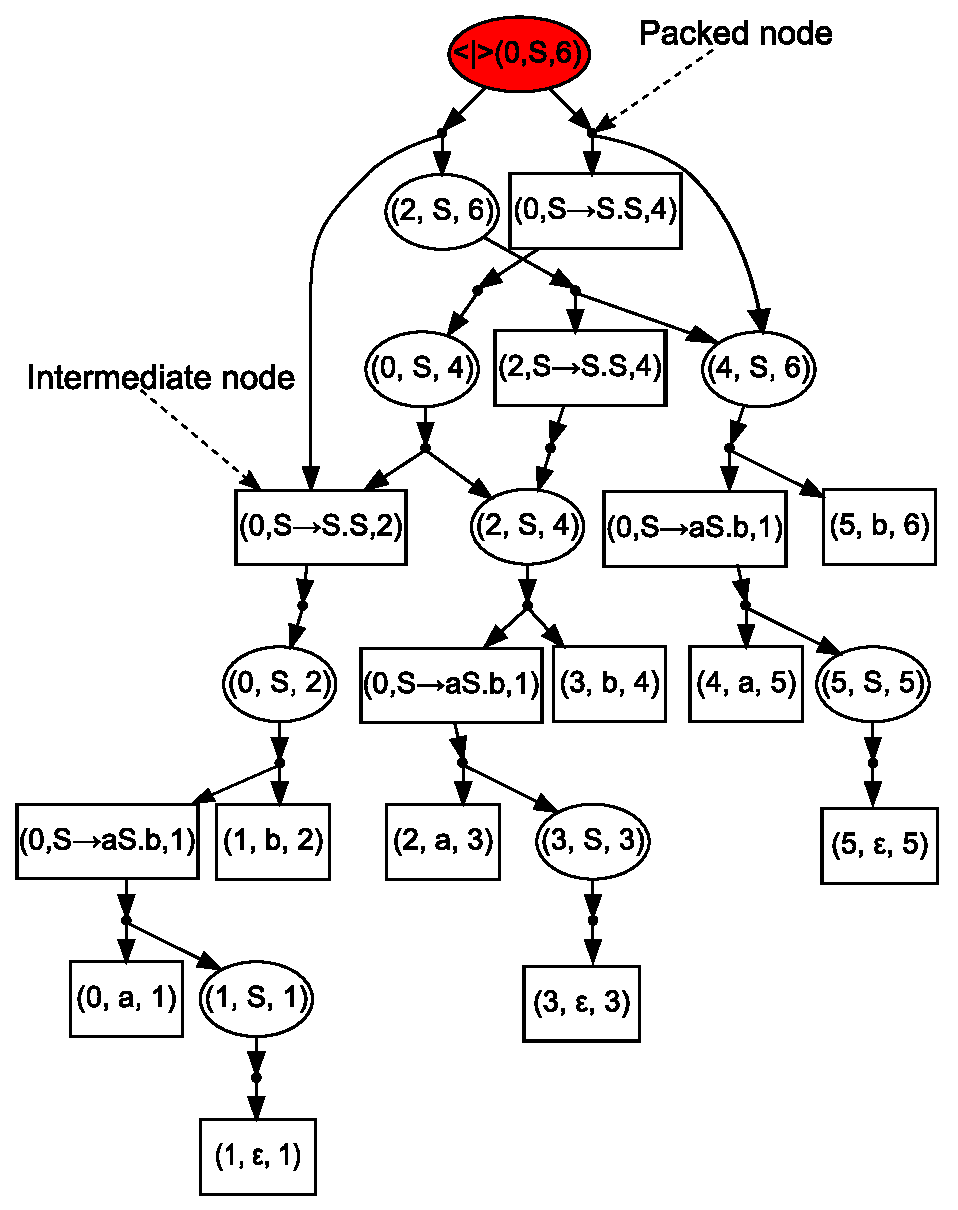
\includegraphics[width=\textwidth]{dot/Brackets.pdf}
        \caption{SPPF}
        \label{sppf}        
    \end{subfigure}
    ~
    \begin{subfigure}[b]{0.3\textwidth}
        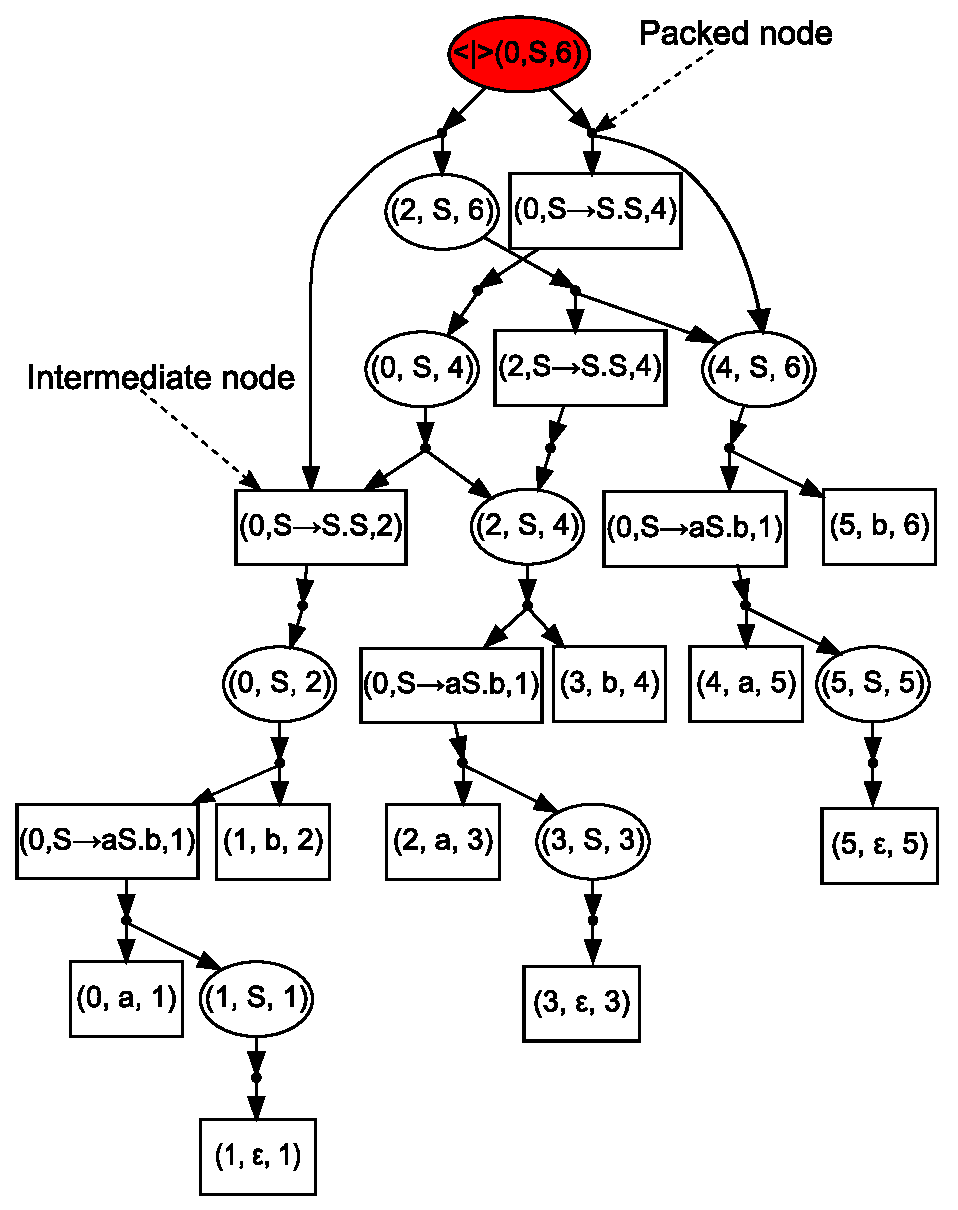
\includegraphics[width=\textwidth]{dot/Brackets.pdf}
        \caption{Tree for derivation 1}
        \label{tree1}        
    \end{subfigure}
    ~
    \begin{subfigure}[b]{0.3\textwidth}
        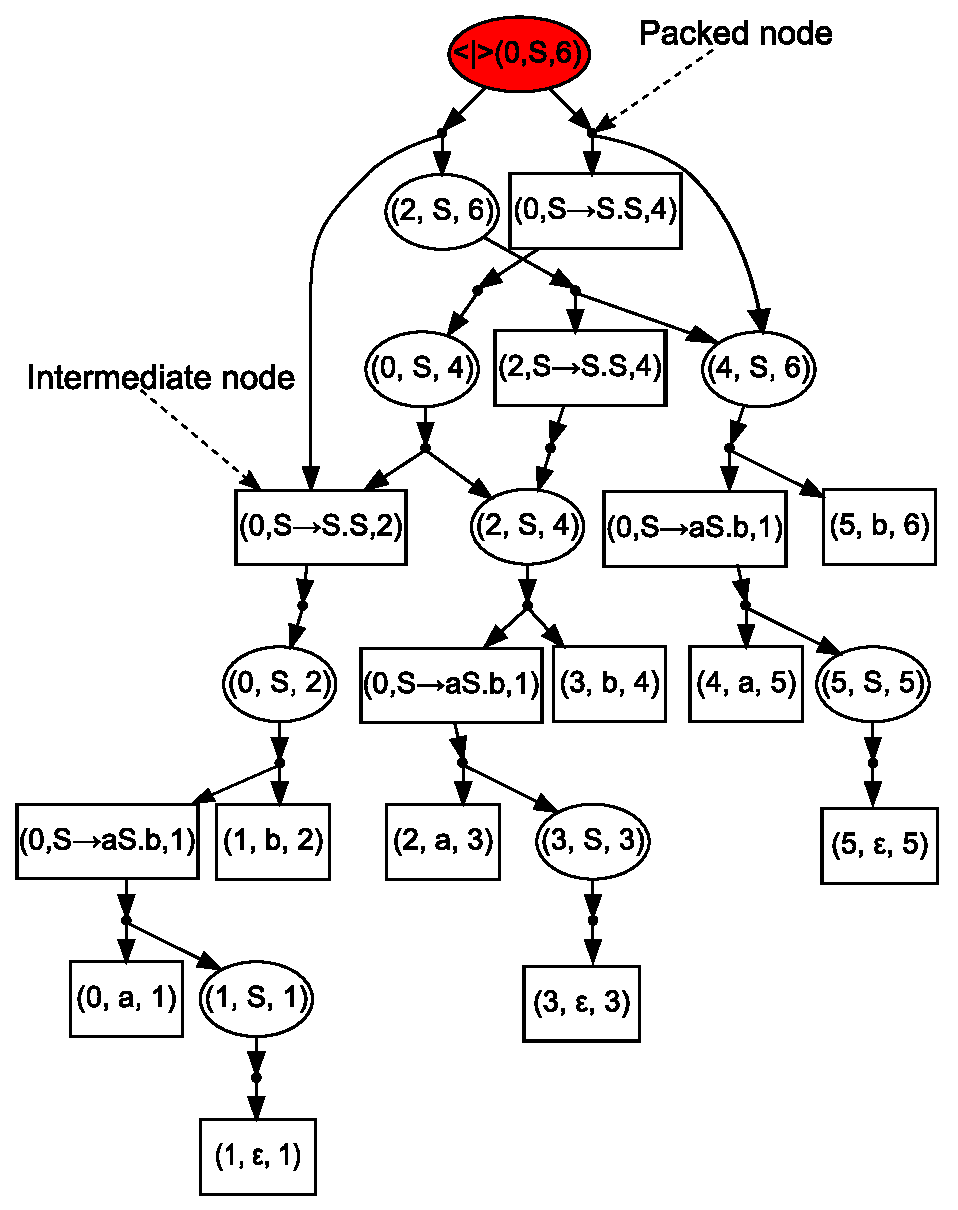
\includegraphics[width=\textwidth]{dot/Brackets.pdf}
        \caption{Tree for derivation 2}
        \label{tree2}        
    \end{subfigure}
    \caption{SPPF for sentence \textbf{\texttt{"(1)(2)(3)"}} and grammar $G_0$}
    \label{sppfSample}
    \end{center}                
\end{figure*}

Binarised SPPF can be represented as a graph where each node has one of four types which described below with corresponded graphical notation.

\begin{itemize}
    \item Node with rectangle shape labeled with $(i, T, j)$ is terminal node.     
    \item Node with oval shape labeled with $(i, N, j)$ is nonterminal node. 
    This node denote that there is at least one derivation for substring $\alpha$ from position $i$ to position $j$ in input string $\omega$ such that $N \Rightarrow^*_G \alpha, \alpha = \omega[i..j-1] $.
    All derivation trees for given substring and nonterminal can be extracted from SPPF by left-to-right top-down graph traversal started from respective node. 
    We use filled nonterminal node labeled with $(<\mkern-11mu | \mkern-11mu> (i, N, j))$ for denote that there are more then one derivations from nonterminal $N$ for substring from $i$ to $j$.
    \item Intermediate node with label $(i,t,j)$ where $t$ is a grammar slot. We use dot shape for these nodes and omit label because it is important only for SPPF constriction.
	Subgraph with root in such node is one variant of derivation in case when parent is nonterminal node with label $(<\mkern-9mu | \mkern-9mu> (i, N, j))$.
    \item Node with rectangle shape and label $(N : \gamma \cdot, k)$ is a packed node.
\end{itemize}
One of nonterminal nodes can be marked as 'root' --- node for start nonterminal. Tuple of positions $(i,j)$ which represent start and end of substring is \textit{extension} of node.

Further in our examples we will remove redundant intermediate and packed nodes from SPPF to simplify it and decrease size of structure.

\subsection{GLL-based graph parsing}

In this section we present such modification of GLL algorithm, that for input graph $M$, set of start vertices $V_s\subseteq V$, set of final vertices $V_f\subseteq V$, grammar $G_1$, it return SPPF which contains all derivation trees for all paths $p$ in $M$, such that $\Omega(p) \in L(G_1)$, and $p.start \in V_s, p.end \in V_f$.

First of all note that input string for classical parser is a linear graph, and positions in input is vertices of this graph.
This observation can be generalized to arbitrary graph with remark that in the position we have not only one next symbol, but set of labels of all outgoing edges for given vertex. 
Thus in order to use GLL for graph parsing we need to use graph vertices as position in input and modify \textbf{Processing} function to allow to process more then one "next symbol".
Required modifications presented in listing~\ref{modifAlgo}.
Small modification also required for initialization of $R$ set: it is necessary to add not only one initial descriptor but set of descriptors for all vertices in $V_s$.
All other functions can be reused from original algorithm without any changes.

\begin{algorithm}[h]
\begin{algorithmic}[1]
\caption{\textbf{Processing} function modified in order to process arbitrary directed graph}
\label{modifAlgo}
\Function{processing}{}
  \State{$dispatch \gets true$}
  \Switch{$L$}
  \Case{$(X \rightarrow \alpha \cdot x \beta)$ where $x$ is terminal}
	   \ForAll{$\{ e | e \in input.outEdges(i), tag(e) = x \}$}
	   \State{$new\_cN \gets cN$}
       \If{$new\_cN = dummyAST$} 
          \State{$new\_cN \gets \Call{getNodeT}{e}$} 
       \Else 
          \State{$new\_cR \gets \Call{getNodeT}{e}$}
       \EndIf
       \State{$L \gets (X \rightarrow \alpha x \cdot \beta)$}
       \If{$new\_cR \neq dummy$}
          \State{$new\_cN \gets \Call{getNodeP}{L, new\_cN, new\_cR}$} 
       \EndIf
	   \State{\Call{add}{L,v,target(e),new\_cN}}
	   \EndFor
  \EndCase
  \Case{$(X \rightarrow \alpha \cdot x \beta)$ where $x$ is nonterminal}
       \State{$v \gets$ \Call{create}{$(X \rightarrow \alpha x \cdot \beta), v, i, cN$}}
       \State{$slots \gets \bigcup_{e \in input.OutEdges(i)} pTable[x][e.Token]$}
       \ForAll{$L \in slots$}
          \State{\Call{add}{L,v,i,dummy}} 
       \EndFor
  \EndCase
  \Case{$(X \rightarrow \alpha \cdot )$}
       \State{\Call{pop}{v,i,cN}} 
  \EndCase
  \Case{$\_$}
       \State{final result processing and error notification} 
  \EndCase
  \EndSwitch
\EndFunction

\end{algorithmic}
\end{algorithm}





As far as we can specify sets of start and final vertices, our solution can find all paths in graph, all paths from specified vertex, all paths between specified vertices. 
Also SPPF represents a structure of paths in terms of derivation which allow to get more useful information about result. 

A bit more on correctness.!!!!!

\subsection{Complexity}

Time complexity estimation in terms of input graph and grammar size is pretty similar to estimation of GLL complexity provided in~\cite{gllParsingTree}.

\begin{lemma}\label{lem:Descriptors}
For any descriptor $(L,u,i,w)$ either $w = \$$ or $w$ has extension $(j,i)$ where u has index $j$.
\end{lemma}
\begin{proof}
Proof of this lemma is the same as provided for original GLL in~\cite{gllParsingTree} because main function used for descriptors creation was not changed.
\end{proof}


\begin{mytheorem}\label{thm:GSSSpace}
The GSS generated by GLL-based graph parsing algorithm for grammar $G$ on input graph $M=(V,E,L)$ has at most $O(|V|)$ vertices and $O(|V|^2)$ edges.
\end{mytheorem}

\begin{proof}

Proof is the same as the proof of \textbf{Theorem 2} from~\cite{gllParsingTree} because structure of GSS was not changed. 

\end{proof}

\begin{mytheorem}\label{thm:SPPFSpace}
The SPPF generated by GLL-based graph parsing algorithm on input graph $M=(V,E,L)$ has at most $O(|V|^3 + |E|)$ vertices and edges.
\end{mytheorem}

\begin{proof}
Let us estimate the number of nodes of each type.
\begin{itemize}
\item \textbf{Terminal nodes.} 
Each of them is labeled with $(T, v_0, v_1)$, and such label can be created only if there is such $e \in E$ that $e=(v_0,T,v_1)$. 
Note, that there are no duplicate edges. 
Hence there are at most $|E|$ terminal nodes.
\item \textbf{$\varepsilon$ nodes} are labeled with $(\varepsilon, v ,v)$, hence there are at most $|V|$ of them. 
\item \textbf{Nonterminal nodes} have labels of form $(N,v_0,v_1)$, so there are at most $O(|V|^2)$ of them.
\item \textbf{Indeterminate nodes} have labels of form $(t,v_0,v_1)$, where $t$ is grammar slot, so there are at most $O(|V|^2)$ of them.
\item \textbf{Packed nodes} are children of intermediate or nonterminal nodes and have label of form $(t,v)$ where $t$ is a grammar slot $N \rightarrow \alpha \cdot \beta$.
There are at most $O(|V|^2)$ parents for packed nodes and each of them can have at most $O(|V|)$ children.
\end{itemize}

As a result there are at most $O(|V|^3 + |E|)$ nodes in SPPF.

The packed nodes have at most two children so there are at most $O(|V|^3 + |E|)$ edges with source in packed node. 
Nonterminal and intermediate nodes have at most $O(|V|)$ children and all of them are packed nodes.
Thus there are at most $O(|V|^3)$ edges with source in nonterminal or intermediate nodes. As a result there are at most $O(|V|^3 + |E|)$ edges in SPPF.


\end{proof}

\begin{mytheorem}
The space complexity of GLL-based graph parsing algorithm for graph $M=(V,E,L)$ is at most $O(|V|^3 + |E|)$.
\end{mytheorem}

\begin{proof}

From theorems~\ref{thm:GSSSpace} and~\ref{thm:SPPFSpace} we have that space required for main data structures is at most $O(|V|^3 + |E|)$. 

\end{proof}


\begin{mytheorem}\label{thm:complexity}
The runtime complexity of GLL-based graph parsing algorithm for graph $M=(V,E,L)$ is at most $$O\left(|V|^3*\max\limits_{v \in V}\left(deg^+\left(v\right)\right)\right).$$
\end{mytheorem}

\begin{proof}

From Lemma~\ref{lem:Descriptors} we get that there are at most $O(|V|^2)$ descriptors. 
Complexity of all functions are the same as in proof of \textbf{Theorem 4} from~\cite{gllParsingTree} except \textbf{Processing} function where we should process not single next input token, but the whole set of outgoing edges.
Thus, for each descriptor we should examine at most $$\max\limits_{v \in V}\left(deg^+\left(v\right)\right)$$ edges where $deg^+(v)$ is outdegree of vertex $v$.

Thus, worst-case complexity of proposed algorithm is $$O\left(V^3*\max\limits_{v \in V}\left(deg^+\left(v\right)\right)\right).$$
\end{proof}

%Also we can get averege-case complexity by calculate averege outdegree:
%\begin{align} \label{eq:avg}
%  & O\left(|V|^3*\frac {\sum\limits_{v \in V} deg^+(v)}{|V|}\right) = \nonumber \\
%  & O\left(|V|^2*\sum\limits_{v \in V} deg^+(v)\right) = \nonumber \\
%  & O\left(|V|^2*|E|\right) 
%\end{align}

From theorem~\ref{thm:complexity} we can get estimations for linear input and for LL grammars: $\text{for any } v \in V$ it is true, that $deg^+(v) \leq 1$, so $\max\limits_{v \in V}(deg^+(v))  = 1 $ and we get $O(|V|^3)$, as expected. 
For LL grammars and linear input complexity should be $O(|V|)$ for the same reason as for original GLL.
 

As discussed in~\cite{modellingGLL} achieving of theoretical complexity required special data structures which can be irrational for practice implementation and it is necessary to find balance between performance, software complexity, and hardware resources.
As a result in practice we can get slightly worse performance than theoretical estimation.

Note that result SPPF contains only paths matched specified query, so result SPPF size is $O(|V'|^3 + |E'|)$ where $M'=(V',E',L')$ is a subgraph of input graph $M$ which contains only matched paths.
Also note that each specific path can be explored with linear SPPF traversal. 

\section{An Example}\label{motivExample}

In this section we ....!!!!!!
We perform classical context-free \textit{same-generation queries}~\cite{FndDB}, which, for example, is an important part of similarity query to biomedical databases~\cite{GraphQueryWithEarley}.

Suppose that you are student in a School of Magic.
It is your first day at School, so navigation in the building is a problem for you.
Fortunately, you have a map of the building (fig.~\ref{input}) and additional knowledge about building construction:
\begin{itemize}
  \item there are towers in the school (depicted as nodes of the graph in your map);
  \item towers can be connected by one-way galleries (represented as edges in your map);
  \item galleries have a ``magic'' property: you can start from any floor, but by following each gallery you either end up one floor above (edge label is `a'), or one floor below (edge label is `b'). 
\end{itemize}

\begin{figure}[h]
    \begin{center}
	\centering
    \begin{subfigure}[b]{0.45\textwidth}
        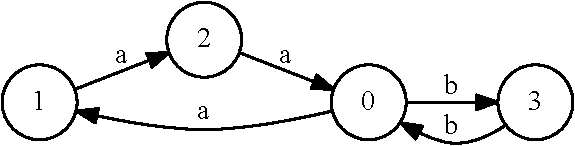
\includegraphics[width=\textwidth]{dot/input.pdf}
        \caption{The map of School (input graph $M$)}
        \label{input}        
		\vspace{1cm}
	\end{subfigure}
	~	
	\begin{subfigure}[b]{0.45\textwidth}
   \[
\begin{array}{rl}
   0:& S \rightarrow a \ S \ b \\
   1:& S \rightarrow Middle \\
   2:& Middle \rightarrow a \ b
\end{array}
\]
   \caption{Grammar $G_1$ for language $L=\{a^n b^n; n \geq 1\}$ with additional marker for the middle of a path}
   \label{grammarG}        
	\end{subfigure}
    \end{center}
\caption{An example: input graph and grammar}
\label{exampleData}
\end{figure}


You want to find a path from your current position to the same floor in another tower. 
Map with all such paths can help you.
But orienteering is not your forte, so it would be great if the structure of the paths were as simple as possible and all paths had additional checkpoints to control your rout.

It is evident that the simplest structure of required paths is $\{ab, aabb, aaabbb, \dots\}$.
In terms of our definitions, it is necessary to find all paths $p$ such that $\Omega(p) \in \{a^n b^n, n \geq 1\}$ in the graph $M=(\{0;1;2;3\},E,\{a;b\})$ (figure~\ref{input}).

Unfortunately, language $\mathcal{L} = \{a^n b^n; n \geq 1\}$ is not regular which restricts the set of tools you can use. 
Another problem is the infinite size of solution, but, being incapable to comprehend an infinite set of paths, you want to get a finite map.  
Moreover, you want to know structure of paths in terms of checkpoints.

We are not aware of any existing tools which can solve this problem, thus we have created such tool.
Let us show how to get a map which helps to navigate in this strange School.

Fortunately, the language $\mathcal{L} = \{a^n b^n; n \geq 1\}$ is a context-free language and it can be specified with context-free grammar. 
The fact that one language can be described with multiple grammars allows to add checkpoints: additional nonterminals can mark required parts of sentences.
In our case, desired checkpoint can be in the middle of the path.
As a result, required language can be specified by the grammar $G_1$ presented in figure~\ref{grammarG}, where $N = \{s; \text{\textit{Middle}}\}$, $\Sigma = \{a; b\}$, and $S$ is a start nonterminal.

Now, let us show that SPPF can be a solution for this problem.
SPPF for data from example is presented in figure~\ref{SPPF}.
Each terminal node corresponds to the edge in the input graph: for each node with label $(v_0, T, v_1)$ there is $e\in E: e=(v_0,T,v_1)$.
Extensions stored in SPPF nodes allow us to check whether path from $u$ to $v$ exists and to extract it by SPPF traverse. 

\begin{figure*}[ht]
    \begin{center}
    \centering
    \begin{subfigure}[b]{0.3\textwidth}
         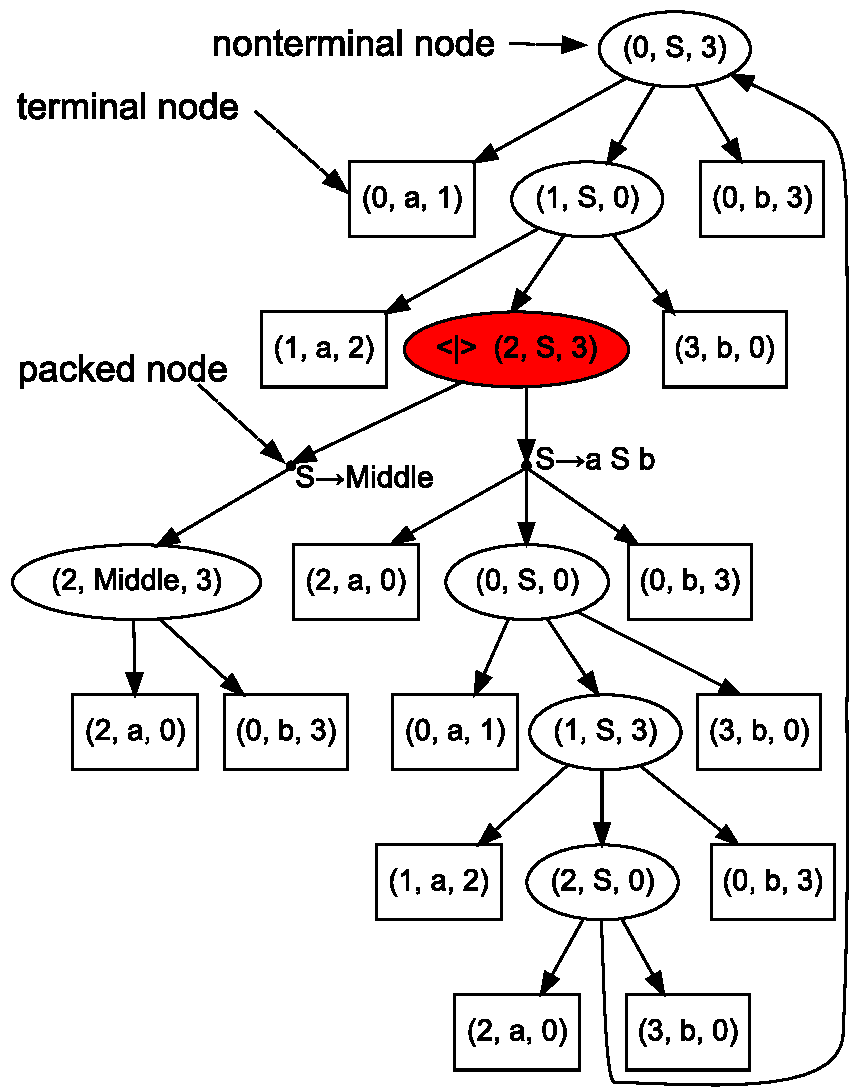
\includegraphics[width=\textwidth]{dot/AnBn.pdf}
        \caption{Result SPPF}
        \label{SPPF}        
    \end{subfigure}
    ~
    \begin{subfigure}[b]{0.3\textwidth}
        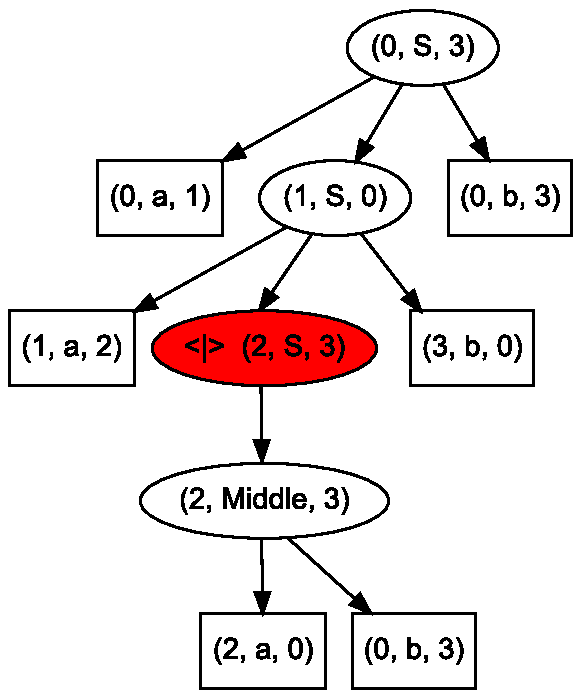
\includegraphics[width=\textwidth]{dot/AnBn_2.pdf}
        \caption{Derivation tree for $p_0$}
        \label{tree1}        
    \end{subfigure}
    ~
    \begin{subfigure}[b]{0.3\textwidth}
        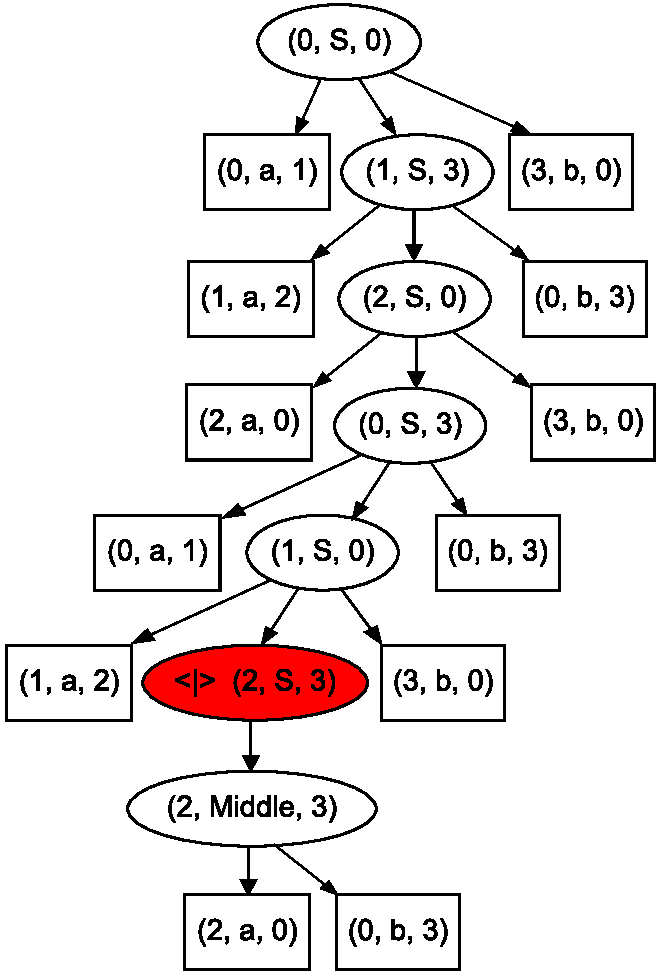
\includegraphics[width=\textwidth]{dot/AnBn_1.pdf}
        \caption{Derivation tree  for $p_1$}
        \label{tree2}        
    \end{subfigure}
    \caption{SPPF and examples of trees for specific paths for data from example (fig~\ref{exampleData}). Presented version does not contains redundant nodes, and we duplicate terminal nodes only for figure simplification.
    We use filled shape and label of form $(<\mkern-11mu | \mkern-11mu> (i, N, j))$ for nonterminal node to denote that there are multiple derivations from nonterminal $N$ for substring $\omega[i..j-1]$.	
	%\\
	%$p_0=\{(0,a,1);(1,a,2);(2,a,0);(0,b,3);(3,b,0);(0,b,3)\}$  \\
    %$p_1=\{(0,a,1);(1,a,2);(2,a,0);(0,a,1);(1,a,2);(2,a,0);(0,b,3);(3,b,0);(0,b,3);\\(3,b,0);(0,b,3);(3,b,0)\}.$
}
    \label{sppfSample}
    \end{center}                
\end{figure*}

As an example of derivation structure usage, we can find a middle of any path in example simply by finding correspondent nonterminal \textit{Middle} in SPPF.
So we can find out that there is only one (common) middle for all results, and it is a vertex with $id = 0$.

Lets find paths $p_i$ such that $S {\xRightarrow[G_1]{}}^{*} \Omega(p_i)$ and $p_i$ starts from the vertex $0$.
To do this, we should find vertices with label $(0, S, \_)$ in SPPF.
(There are two vertices with such labels: $(0, S, 0)$ and $(0, S, 3)$.)
Then let us to extract corresponded paths from SPPF.
There is a cycle in SPPF in our example, so there are \textbf{at least} two different paths: $p_0=\{(0,a,1);(1,a,2);(2,a,0);(0,b,3);(3,b,0);(0,b,3)\}$ and 
$
p_1=\{(0,a,1);(1,a,2);(2,a,0);(0,a,1);(1,a,2);(2,a,0);(0,b,3);(3,b,0);(0,b,3);\\(3,b,0);(0,b,3);(3,b,0)\}.
$ Trees for these paths are presented in figures~\ref{tree1} and~\ref{tree2} respectively.
%\end{align*}

We demonstrate that SPPF which was constructed by described algorithm can be useful for query result investigation. 
But in some cases explicit representation of matched subgraph is preferable, and required subgraph may be extracted from SPPF trivially by its traversal.

In order to test the resulting solution we have implemented the frontend as a plugin using ReSharper SDK, so it can be installed into ReSharper, Rider and InspectCode.
The source code is parsed by internal ReSharper tools and the result is used to produce graphs and meta-information.
The issues found by the backend are shown using code highlighting.

The first analysis which has been implemented is the considered taint tracking analysis.
It is defined just by the PDA constructed in the section 2 translated into the code with some slight modifications which make it possible to process interactions with object fields.
To provide more information about an issue found by this analysis, the higlighting is accompanied by bulbs containing the full path of tainted variable from the source to the sink represented as the sequence of operations.

\subsection{Sample cases}

Let's look closer at properties of the resulting soluiton.
All these properties are illustrated by screenshots taken exactly from the runned Rider IDE with some small relocations of bulbs to make them not to overlap the code.

Firstly, the solution ensures flow sensitivity. I.e. it processes flow of variables passed into methods and returned from them correctly.
Which can be seen at fig~\ref{fig:ReturnsAndBrackets}.
This example illustrates the most common cases of interprocedural data passing.
\textit{Brackets} method gets the data, performs some computations on them and returns the result.
Invocations at lines 37 and 38 shows that the solution can distinguish two data flow paths despite both of them passes through the same method.
So, \textit{e} becomes tainted because \textit{c} is tainted and \textit{f} does not because \textit{d} is clear.
Moreover, the solution can track paths where passes and returns do not form the correct bracket sequence that is shown by method \textit{PostSource} which does not take any parameter and just returns tainted data.

\begin{figure}[h]
	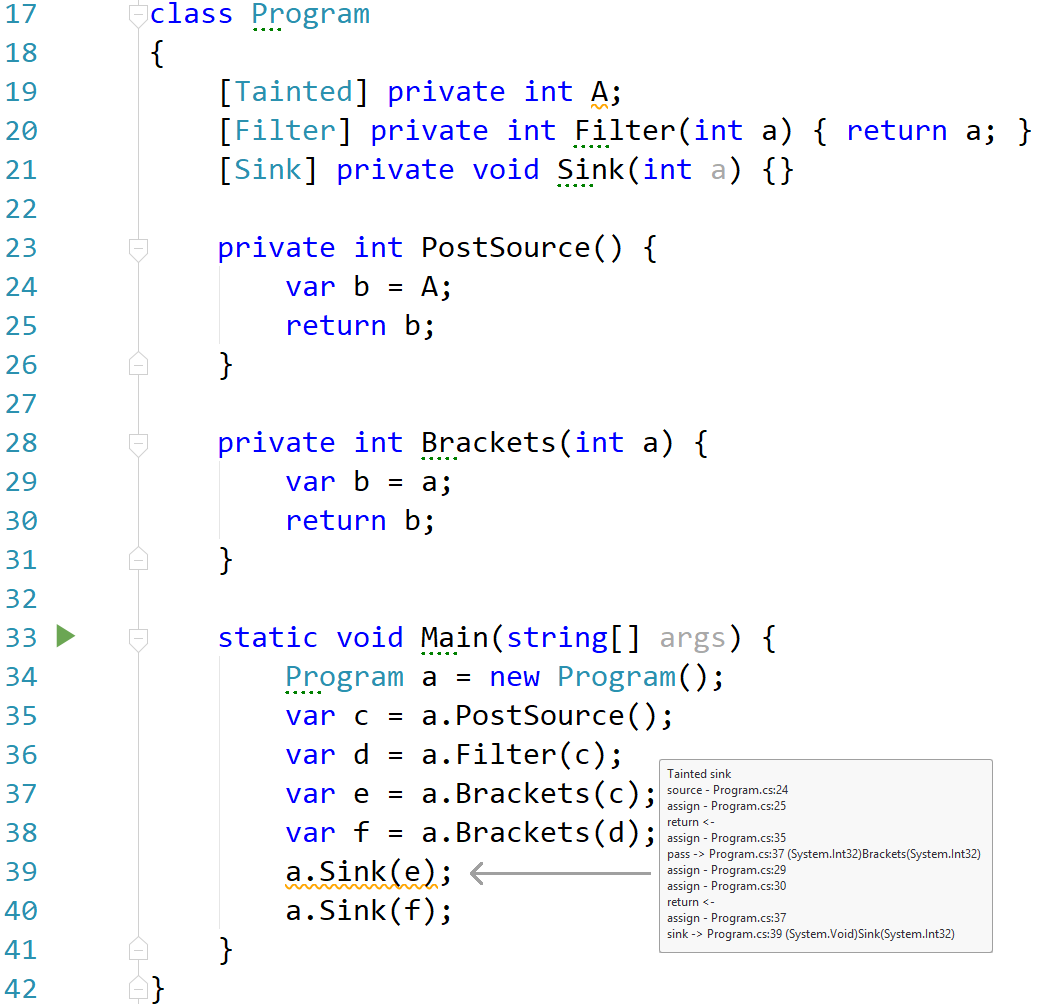
\includegraphics[width=\linewidth]{screenshots/ReturnsAndBrackets.png}
	\caption{Flow sensitivity}
	\label{fig:ReturnsAndBrackets}
\end{figure}

Secondly, the solution has the limited context sensitivity. I.e. it allows to track propagation of objects that are tainted by assigning of some fields inside them both by their own methods and by outer code interacting with their fields directly.
The first case is shown at fig~\ref{fig:ObjectTainting}.
There is the field \textit{B} at the line 18. 
This field can be used widely in the logic of the \textit{Container} class and by this the tainting of this field is considered as the tainting of the whole object.
However, while processing of the method \textit{Store} during the analysis it is hard to decide what the object need to be tainted because in the inner context of \textit{Store} it is just \textit{this} object.
I.e. we must consider the calling context to make such decision.
So, the solution provides this opportunity which is shown by lines 33-36 where the first invocation of \textit{Store} leads to the tainting of object \textit{d} and the second invocation does not taint object \textit{e}.

\begin{figure}[h]
	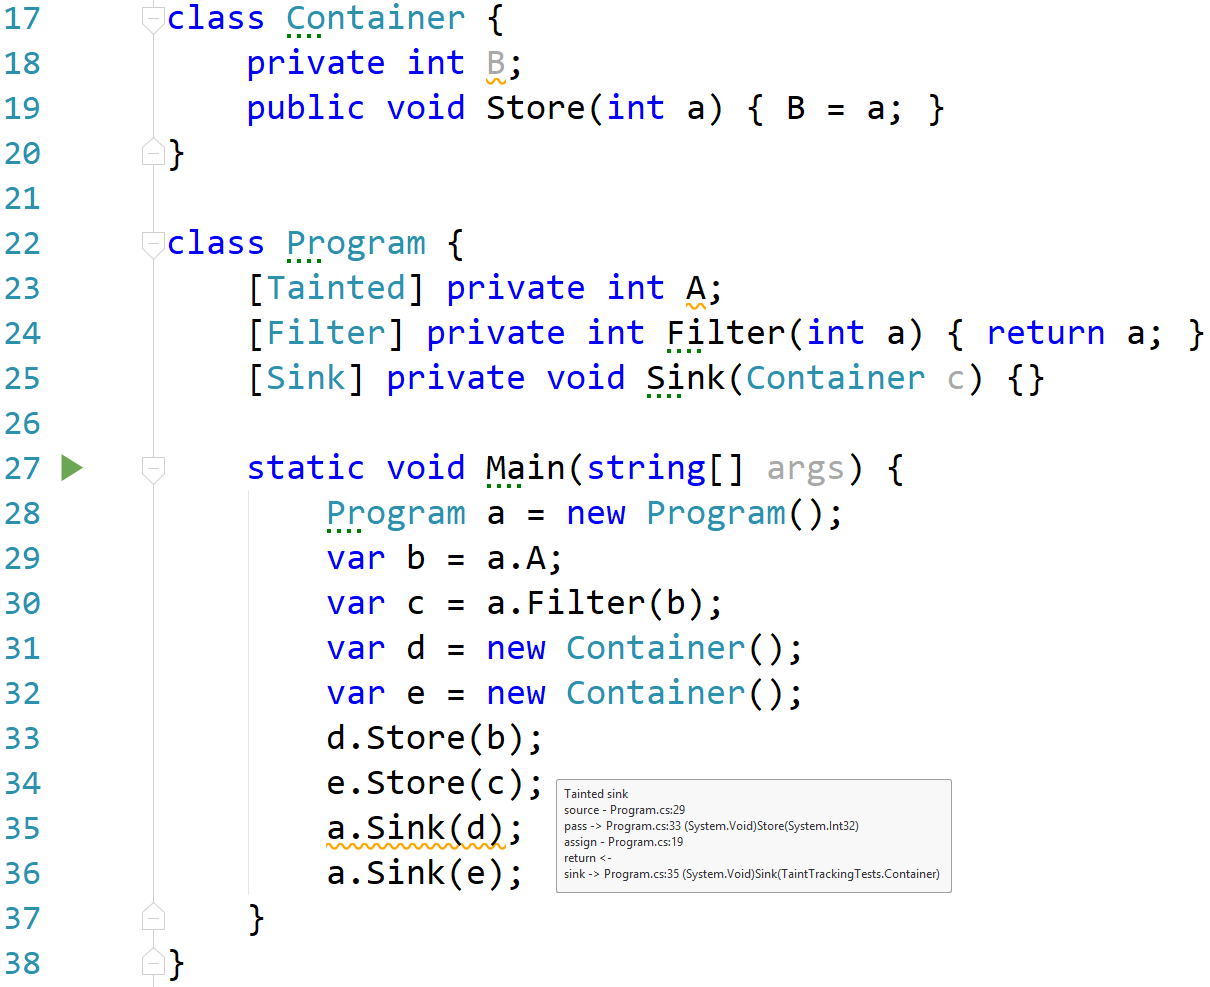
\includegraphics[width=\linewidth]{screenshots/ContextSensitivity.png}
	\caption{Tainting of an object by its own method}
	\label{fig:ObjectTainting}
\end{figure}

Finally, the solution works with any type of recursion and does not fall into infinite cycles.
It can be seen at fig.~\ref{fig:Recursion}.
This snippet contains two mutually recursive methods which pass the data to each other.
The solution checks all possible paths of passing even those which includes cyclic invocations and returns the passed variable to the point corresponding to the initial invocation.

\begin{figure}[h]
	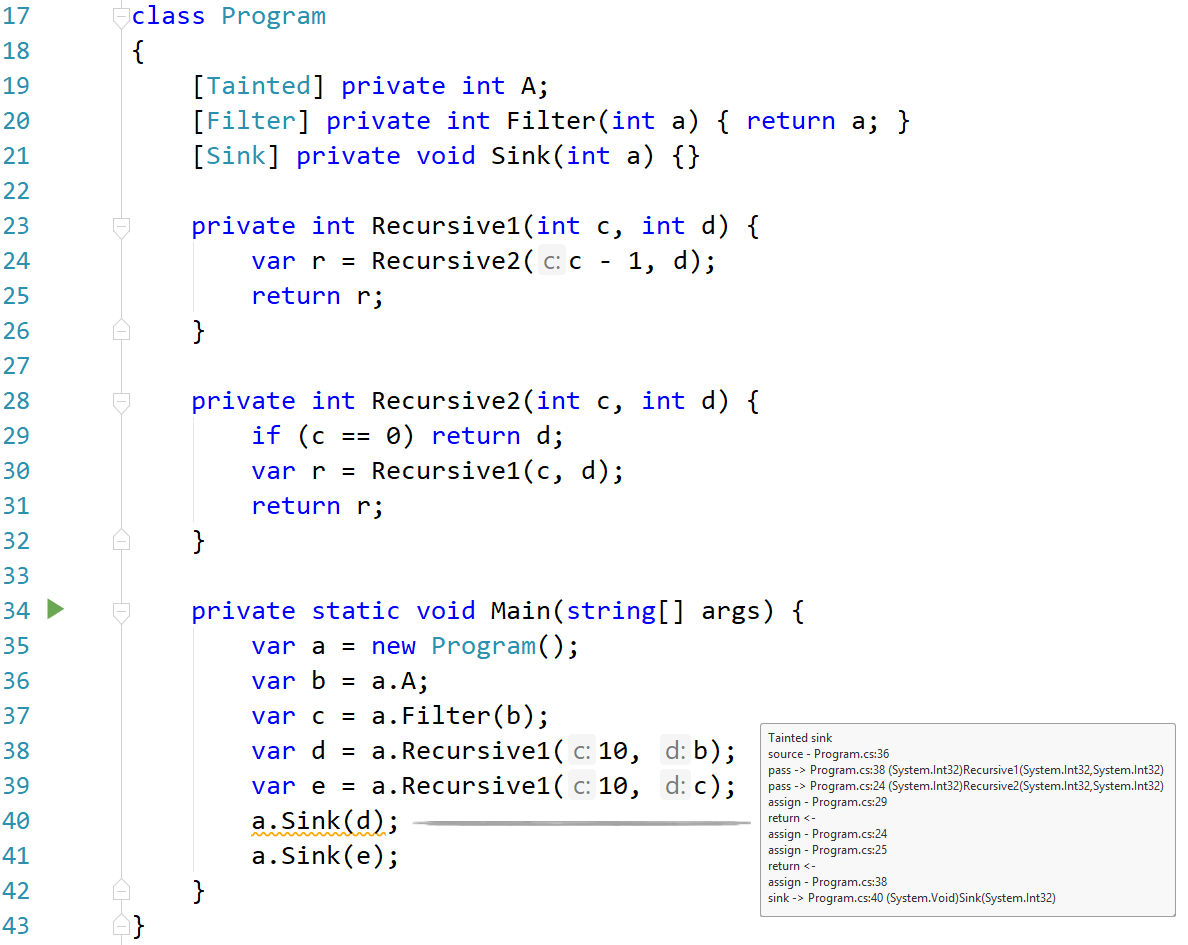
\includegraphics[width=\linewidth]{screenshots/Recursion.png}
	\caption{Recursive methods processing}
	\label{fig:Recursion}
\end{figure}

\subsection{Performance}

It is also necessary to measure the performance of the resulting solution.
Because the implemented taint tracking analysis forces to mark all participating entities manually, it is difficult to perform it on some large project.
However, there is another intermediate analysis which is runned before any other one to collect some information required by resolver.
In particular, it tracks propagation of all variables to discover all possible concrete types of each variable.
So, it involves each variable and each method in the whole program and thus the time and space required for execution of this analysis may be consistent estimation of the efficiency of the solution.

The code base that has been chosen as a source of data is the full solution of the Mono project.
(TODO: ADD SYSTEM CONFIGURATION).
The results is shown in the table~\ref{tab:Performance}.

\begin{table}[h]
	\begin{tabular}{|l|l|l|l|l|}
	\hline
		Project & Classes & Methods & \begin{tabular}[c]{@{}l@{}}Execution \\ time (s)\end{tabular} & \begin{tabular}[c]{@{}l@{}}Allocated \\ memory (GB)\end{tabular} \\ \hline
		Mono & 21013 & 192745 & $21\pm 0.5$ & $\sim 4.2$ \\ \hline
	\end{tabular}
	\caption{Performance}
	\label{tab:Performance}
\end{table}

\section{Conclusion}

We propose and implement in C\# programming language the generic framework for interprocedural static code analysis implementation.
This framework allows one to implement arbitrary interprocedural analysis in terms of CFL-reachability.
By using the proposed framework, we implement a plugin upon ReSharper infrastructure which provides simple taint analysis and demonstrate that our solution can handle important real-world cases.
Also we show that the proposed framework can be used for real-world solutions analysis.

One of the directions for future work is a creation of analysis and its evaluation on real-world projects.
By this way, we want to get information which helps to improve the usability of our framework: tune performance, improve API, etc.
Also we should improve documentation and create more examples of usage.

Another direction is a practical evaluation of automatic fix location prediction by using minimum cuts method~\cite{10.1007/978-3-319-63390-9_27}.

Also we want to compare the proposed approach with other generic CFL-reachability based approaches for interprocedural code analysis cretion. For example, fith generation-based approach~\cite{LPAR-21:Cauliflower_Solver_Generator_for}, which idea is similar to parser generators.

\section*{Acknowledgments}

Jelle Hellings

Ekaterina Verbitskaia

JetBrains

etal



\bibliographystyle{ACM-Reference-Format}
\bibliography{ContextFreeConstrainedPathFindingInGraph} 

\end{document}
